\newpage

\section{Tinjauan Pustaka}

\subsection{EDA (Exploratory Data Analysis)}
% Buat tinjauan pustaka untuk EDA gunakan refrensi yang relevan
Exploratory Data Analysis (EDA) adalah proses analisis data yang bertujuan untuk memahami struktur, pola, dan hubungan dalam dataset sebelum menerapkan model statistik atau machine learning. EDA melibatkan visualisasi data, statistik deskriptif, dan identifikasi anomali atau outlier. Proses ini penting untuk mendapatkan wawasan awal tentang data dan membantu dalam pengambilan keputusan selanjutnya.

\subsection{Regresi Linier}
% Buat tinjauan pustaka untuk regresi linier gunakan refrensi yang relevan
Regresi linier adalah metode statistik yang digunakan untuk memodelkan hubungan antara satu atau lebih variabel independen (fitur) dengan variabel dependen (target). Model ini mengasumsikan bahwa hubungan antara variabel-variabel tersebut dapat direpresentasikan sebagai garis lurus. Regresi linier sering digunakan dalam analisis data untuk prediksi dan inferensi, serta merupakan dasar bagi banyak algoritma machine learning lainnya.

%buat kata kata pengantar untuk bisa membawa rumus regresi linier
Agar dapat memahami bagaimana regresi linier bekerja, kita perlu memahami rumus dasar dari regresi linier. Regresi linier sederhana melibatkan satu variabel independen, sedangkan regresi linier berganda melibatkan beberapa variabel independen. Dalam tugas ini, kita akan fokus pada regresi linier berganda untuk memprediksi jumlah penonton video Youtube berdasarkan metadata yang tersedia.

%masukan rumus regresi linier untuk pemodelan
\begin{equation}
    y = \beta_0 + \beta_1 x_1 + \beta_2 x_2 + ... + \beta_n x_n + \epsilon
\end{equation}

%jelaskan masing masing variabel
Di mana:
\begin{itemize}
    \item $y$ adalah variabel dependen (target).
    \item $\beta_0$ adalah intercept (nilai awal ketika semua variabel independen bernilai nol).
    \item $\beta_1, \beta_2, ..., \beta_n$ adalah koefisien regresi yang menunjukkan pengaruh masing-masing variabel independen terhadap variabel dependen.
    \item $x_1, x_2, ..., x_n$ adalah variabel independen (fitur).
    \item $\epsilon$ adalah error term yang mencakup variasi yang tidak dijelaskan oleh model.
\end{itemize}

%jelaskan kecanggihan teknologi sehingga memudahkan penggunaan regresi linier dalam model machine learning

Dengan kemajuan teknologi dan ketersediaan pustaka machine learning yang kuat seperti scikit-learn, TensorFlow, dan PyTorch, penerapan regresi linier dalam model machine learning menjadi lebih mudah dan efisien. Pustaka-pustaka ini menyediakan fungsi-fungsi yang memungkinkan pengguna untuk dengan cepat membangun, melatih, dan mengevaluasi model regresi linier tanpa harus mengimplementasikan algoritma dari awal.

\subsection{Ridge Regression}
% Buat tinjauan pustaka untuk ridge regression gunakan refrensi yang relevan
Ridge regression adalah teknik regresi linier yang digunakan untuk mengatasi masalah multikolinearitas, yaitu ketika dua atau lebih variabel independen sangat berkorelasi satu sama lain. Ridge regression menambahkan penalti pada ukuran koefisien regresi untuk mengurangi kompleksitas model dan mencegah overfitting. Penalti ini dihitung sebagai kuadrat dari norma L2 dari koefisien regresi, sehingga menghasilkan model yang lebih stabil dan generalisasi yang lebih baik pada data baru.

\begin{equation}
    \text{Ridge Loss} = \sum_{i=1}^{n} (y_i - \hat{y}_i)^2 + \lambda \sum_{j=1}^{p} \beta_j^2
\end{equation}
Di mana:
\begin{itemize}
    \item $n$ adalah jumlah data.
    \item $y_i$ adalah nilai aktual.
    \item $\hat{y}_i$ adalah nilai yang diprediksi oleh model.
    \item $\lambda$ adalah parameter regularisasi yang mengontrol kekuatan penalti.
    \item $p$ adalah jumlah variabel independen.
    \item $\beta_j$ adalah koefisien regresi untuk variabel independen ke-$j$.
    \item $\sum_{j=1}^{p} \beta_j^2$ adalah penalti L2 yang ditambahkan ke fungsi loss untuk mengurangi kompleksitas model.
\end{itemize}

\subsection{Lasso Regression}
% Buat tinjauan pustaka untuk lasso regression gunakan refrensi yang relevan
Lasso Regression adalah teknik regresi linier yang juga digunakan untuk mengatasi masalah multikolinearitas, tetapi dengan pendekatan yang berbeda dibandingkan dengan Ridge Regression. Lasso Regression menambahkan penalti pada ukuran koefisien regresi menggunakan norma L1, yang dapat menghasilkan koefisien regresi nol untuk beberapa variabel independen. Hal ini memungkinkan Lasso Regression melakukan seleksi fitur secara otomatis, sehingga menghasilkan model yang lebih sederhana dan interpretatif.
\begin{equation}
    \text{Lasso Loss} = \sum_{i=1}^{n} (y_i - \hat{y}_i)^2 + \lambda \sum_{j=1}^{p} |\beta_j|
\end{equation}
Di mana:
\begin{itemize}
    \item $n$ adalah jumlah data.
    \item $y_i$ adalah nilai aktual.
    \item $\hat{y}_i$ adalah nilai yang diprediksi oleh model.
    \item $\lambda$ adalah parameter regularisasi yang mengontrol kekuatan penalti.
    \item $p$ adalah jumlah variabel independen.
    \item $\beta_j$ adalah koefisien regresi untuk variabel independen ke-$j$.
    \item $\sum_{j=1}^{p} |\beta_j|$ adalah penalti L1 yang ditambahkan ke fungsi loss untuk mengurangi kompleksitas model dan melakukan seleksi fitur.
    \item $|\beta_j|$ adalah nilai absolut dari koefisien regresi untuk variabel independen ke-$j$.
\end{itemize}

\subsection{Random Forest Regression}
% Buat tinjauan pustaka untuk random forest regression gunakan refrensi yang relevan
Random Forest Regression adalah metode ensemble learning yang menggabungkan beberapa pohon keputusan untuk meningkatkan akurasi prediksi. Metode ini bekerja dengan membangun sejumlah pohon keputusan pada subset acak dari data pelatihan dan kemudian menggabungkan hasil prediksi dari semua pohon tersebut. Random Forest Regression sangat efektif dalam menangani data dengan banyak fitur dan dapat mengurangi risiko overfitting yang sering terjadi pada pohon keputusan tunggal.
\begin{equation}
    \hat{y} = \frac{1}{T} \sum_{t=1}^{T} f_t(x)
\end{equation}
Di mana:
\begin{itemize}
    \item $\hat{y}$ adalah prediksi akhir dari Random Forest.
    \item $T$ adalah jumlah pohon dalam hutan acak.
    \item $f_t(x)$ adalah prediksi dari pohon keputusan ke-$t$ untuk input $x$.
    \item $\sum_{t=1}^{T} f_t(x)$ adalah jumlah prediksi dari semua pohon keputusan.
    \item $\frac{1}{T}$ adalah rata-rata dari prediksi semua pohon keputusan, yang memberikan hasil akhir dari Random Forest Regression.
    \item $T$ adalah jumlah pohon keputusan yang digunakan dalam Random Forest, yang biasanya ditentukan oleh pengguna sebagai hyperparameter.
\end{itemize}


\subsection{Metadata Youtube}
% Buat tinjauan pustaka untuk metadata Youtube gunakan refrensi yang relevan
Metadata Youtube mencakup berbagai informasi yang terkait dengan video, seperti judul, deskripsi, tag, kategori, dan statistik penonton. Metadata ini sangat penting karena membantu algoritma Youtube dalam merekomendasikan video kepada pengguna dan mempengaruhi visibilitas video di platform. Dengan menganalisis metadata, kita dapat mengidentifikasi faktor-faktor yang berkontribusi terhadap popularitas video dan mengembangkan strategi untuk meningkatkan performa konten.

\begin{figure}[ht]
    \centering
    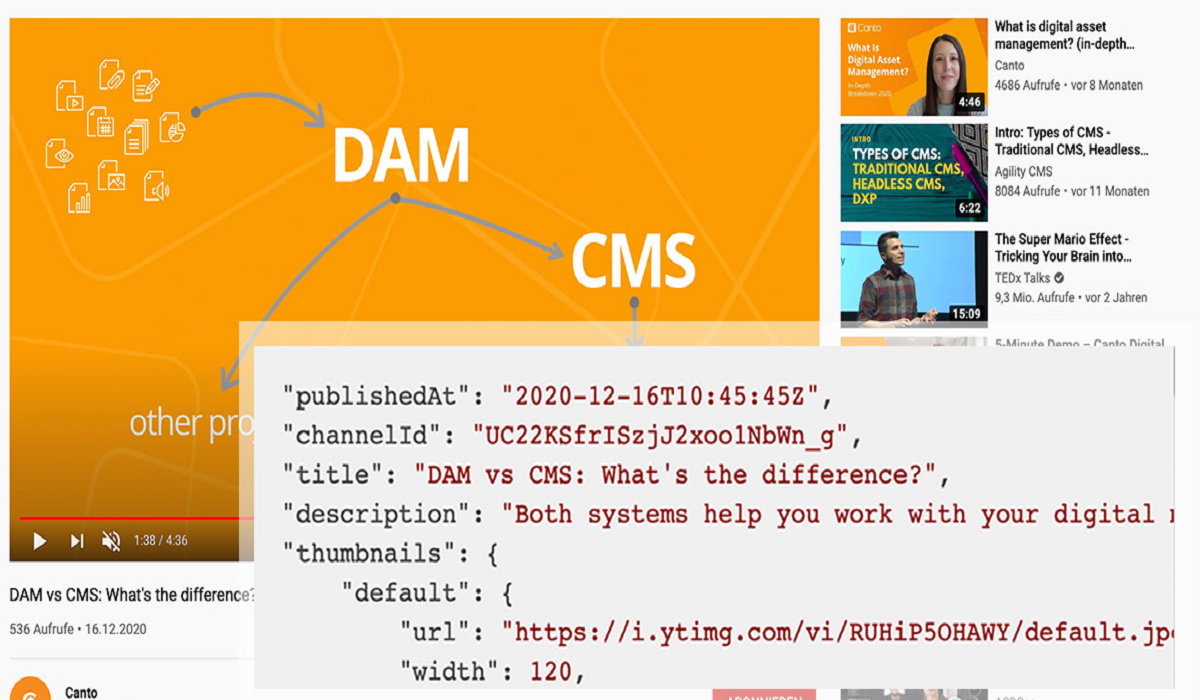
\includegraphics[width=0.8\textwidth]{gambar/youtube-metadata.png}
    \caption{Contoh Metadata Youtube}
    \label{fig:metadata_youtube}
\end{figure}

\subsection{RMSE (Root Mean Square Error)}
% Buat tinjauan pustaka untuk RMSE gunakan refrensi yang relevan
Root Mean Square Error (RMSE) adalah metrik evaluasi yang digunakan untuk mengukur seberapa baik model prediksi dalam memprediksi nilai-nilai numerik. RMSE menghitung akar kuadrat dari rata-rata kuadrat selisih antara nilai yang diprediksi dan nilai aktual. Metrik ini memberikan gambaran tentang seberapa besar kesalahan prediksi model, dengan semakin kecil nilai RMSE menunjukkan performa model yang lebih baik.

\begin{equation}
    RMSE = \sqrt{\frac{1}{n} \sum_{i=1}^{n} (y_i - \hat{y}_i)^2}
\end{equation}

Di mana:
\begin{itemize}
    \item $n$ adalah jumlah data.
    \item $y_i$ adalah nilai aktual.
    \item $\hat{y}_i$ adalah nilai yang diprediksi oleh model.
\end{itemize}

\subsection{$R^2$ (Koefisien Determinasi)}
% Buat tinjauan pustaka untuk $R^2$ gunakan refrensi yang relevan
Koefisien Determinasi ($R^2$) adalah metrik yang digunakan untuk mengukur seberapa baik model regresi menjelaskan variasi dalam data. Nilai $R^2$ berkisar antara 0 hingga 1, di mana nilai yang lebih tinggi menunjukkan bahwa model mampu menjelaskan proporsi yang lebih besar dari variasi dalam data. Metrik ini sering digunakan untuk mengevaluasi performa model regresi dan membandingkan model yang berbeda.

\begin{equation}
    R^2 = 1 - \frac{\sum_{i=1}^{n} (y_i - \hat{y}_i)^2}{\sum_{i=1}^{n} (y_i - \bar{y})^2}
\end{equation}

Di mana:
\begin{itemize}
    \item $n$ adalah jumlah data.
    \item $y_i$ adalah nilai aktual.
    \item $\hat{y}_i$ adalah nilai yang diprediksi oleh model.
    \item $\bar{y}$ adalah rata-rata dari nilai aktual.
\end{itemize}

\subsection{Modeling}
% Buat tinjauan pustaka untuk modeling gunakan refrensi yang relevan
Modeling dalam konteks machine learning adalah proses membangun model matematis atau statistik yang dapat digunakan untuk membuat prediksi atau mengambil keputusan berdasarkan data. Proses ini melibatkan pemilihan algoritma, pelatihan model dengan data, dan evaluasi performa model menggunakan metrik yang relevan. Dalam tugas ini, kita akan fokus pada penerapan regresi linier sebagai metode modeling utama untuk memprediksi jumlah penonton video Youtube berdasarkan metadata yang tersedia.

\subsection{Scikit-learn}
% Buat tinjauan pustaka untuk scikit-learn gunakan refrensi yang relevan
Scikit-learn adalah pustaka machine learning yang populer di Python yang menyediakan berbagai algoritma dan alat untuk analisis data dan modeling. Pustaka ini menawarkan antarmuka yang sederhana dan konsisten, sehingga memudahkan pengguna untuk menerapkan berbagai algoritma machine learning, termasuk regresi linier, klasifikasi, clustering, dan lain-lain. Scikit-learn juga menyediakan fungsi-fungsi untuk preprocessing data, evaluasi model, dan validasi silang, menjadikannya pilihan yang ideal untuk proyek-proyek machine learning.

\subsection{Matplotlib dan Seaborn}

% Buat tinjauan pustaka untuk matplotlib dan seaborn gunakan refrensi yang relevan
Matplotlib dan Seaborn adalah pustaka visualisasi data yang populer di Python. Matplotlib menyediakan fungsi dasar untuk membuat berbagai jenis grafik, seperti garis, batang, dan sebar, sedangkan Seaborn adalah ekstensi dari Matplotlib yang menawarkan antarmuka yang lebih tinggi dan lebih mudah digunakan untuk visualisasi statistik. Keduanya sangat berguna dalam proses EDA (Exploratory Data Analysis) untuk memahami struktur dan pola dalam data melalui visualisasi yang informatif.

\subsection{Pandas}

% Buat tinjauan pustaka untuk pandas gunakan refrensi yang relevan
Pandas adalah pustaka Python yang menyediakan struktur data dan fungsi untuk manipulasi dan analisis data. Pustaka ini menawarkan DataFrame, yang merupakan struktur data tabular yang memungkinkan pengguna untuk dengan mudah mengakses, memanipulasi, dan menganalisis data. Pandas sangat berguna dalam proses EDA (Exploratory Data Analysis) karena menyediakan berbagai fungsi untuk membersihkan, mengolah, dan menganalisis data secara efisien.

\subsection{Transform log1p}
% Buat tinjauan pustaka untuk transform log1p gunakan refrensi yang relevan
Transformasi log1p adalah teknik yang digunakan untuk mengatasi masalah distribusi data yang tidak normal, terutama ketika data memiliki nilai nol atau sangat kecil. Fungsi log1p menghitung logaritma dari (1 + x), yang memungkinkan transformasi data positif dan nol tanpa menghasilkan nilai tak terdefinisi. Transformasi ini sering digunakan dalam analisis regresi untuk meningkatkan normalitas residual dan mengurangi pengaruh outlier.

%rumus log1p
\begin{equation}
    \text{log1p}(x) = \log(1 + x)
\end{equation}

Di mana :
\begin{itemize}
    \item $x$ adalah nilai input.
    \item $\log$ adalah fungsi logaritma natural.
\end{itemize}

\subsection{Transform expm1}
% Buat tinjauan pustaka untuk expm1 gunakan refrensi yang relevan
expm1 adalah fungsi yang digunakan untuk menghitung eksponensial dari suatu nilai dikurangi satu, yaitu $e^x - 1$. Fungsi ini berguna dalam konteks transformasi data, terutama ketika bekerja dengan data yang telah ditransformasi menggunakan logaritma. Fungsi expm1 membantu mengembalikan nilai asli dari transformasi logaritma dengan cara yang lebih stabil secara numerik, terutama untuk nilai-nilai kecil.
\begin{equation}
    \text{expm1}(x) = e^x - 1
\end{equation}

Di mana :
\begin{itemize}
    \item $x$ adalah nilai input.
    \item $e$ adalah bilangan Euler (sekitar 2.71828).
\end{itemize}

\subsection{Hyperparameter Tuning}

% Buat tinjauan pustaka untuk hyperparameter tuning gunakan refrensi yang relevan
Hyperparameter tuning adalah proses mencari nilai optimal untuk hyperparameter model machine learning yang tidak dipelajari selama pelatihan. Hyperparameter adalah parameter yang ditentukan sebelum pelatihan dimulai, seperti laju pembelajaran, jumlah pohon dalam hutan acak, atau kedalaman pohon keputusan. Proses ini penting karena pemilihan hyperparameter yang tepat dapat secara signifikan mempengaruhi performa model. Teknik umum untuk hyperparameter tuning termasuk grid search, random search, dan Bayesian optimization.

\subsection{StandardScaler}
% Buat tinjauan pustaka untuk StandardScaler gunakan refrensi yang relevan
StandardScaler adalah kelas dalam pustaka scikit-learn yang digunakan untuk melakukan normalisasi data dengan mengubah distribusi fitur menjadi distribusi normal standar (mean = 0, standar deviasi = 1). Proses ini penting dalam machine learning karena membantu algoritma belajar lebih efektif dengan memastikan bahwa semua fitur memiliki skala yang sama. StandardScaler menghitung mean dan standar deviasi dari setiap fitur pada data pelatihan dan menerapkannya pada data pelatihan dan pengujian.
\begin{equation}
    z = \frac{x - \mu}{\sigma}
\end{equation}
Di mana:
\begin{itemize}
    \item $z$ adalah nilai yang dinormalisasi.
    \item $x$ adalah nilai asli.
    \item $\mu$ adalah mean dari fitur.
    \item $\sigma$ adalah standar deviasi dari fitur.
\end{itemize}

